\section{Visão Geral do Sistema}

\begin{frame}
    \frametitle{Visão Geral do Sistema}

    Quatro etapas principais:

    \begin{itemize}
        \item Obter \alert{informação sobre a fase}
        \item \alert{Detectar a fase} corretamente
        \item \alert{Variação de Frequências} (HMFCW)
        \item \alert{Cálculo da posição 3D}
    \end{itemize}
\end{frame}

\begin{frame}
    \frametitle{Visão Geral do Sistema}

    \begin{center}
        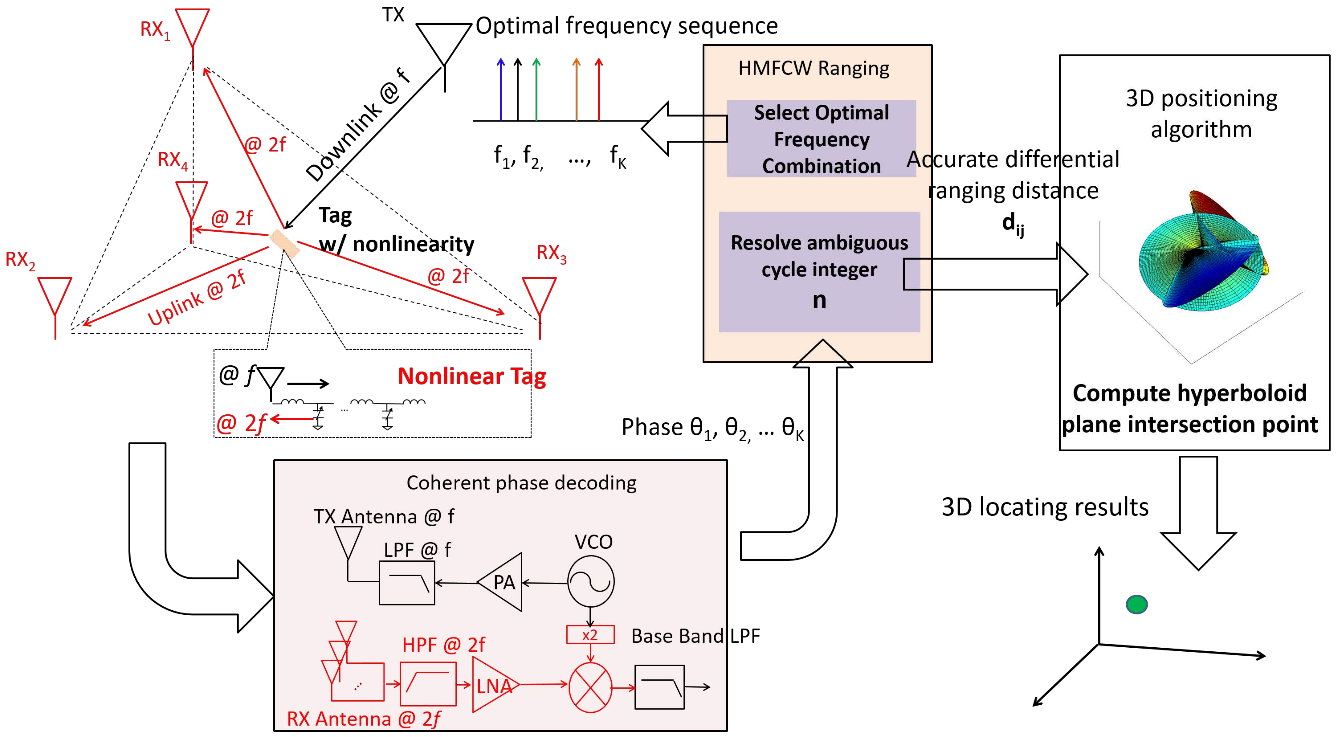
\includegraphics[width=1\textwidth]{overview}
    \end{center}
\end{frame}

\section{Eliminando o Auto-Bloqueio}

\begin{frame}
    \frametitle{Eliminando o Auto-Bloqueio}

    Entendendo o problema:
    \begin{itemize}
        \item Tags RFID consomem \alert{$\approx{}10\mu{}W$}
        \item Não têm energia para \alert{gerar sinais}
        \item Portanto, precisam \alert{refletir o sinal do emissor}
            \pause
        \item \alert{Como saber de onde vem uma reflexão?}
    \end{itemize}
\end{frame}

\begin{frame}
    \frametitle{Eliminando o Auto-Bloqueio}

    \begin{center}
        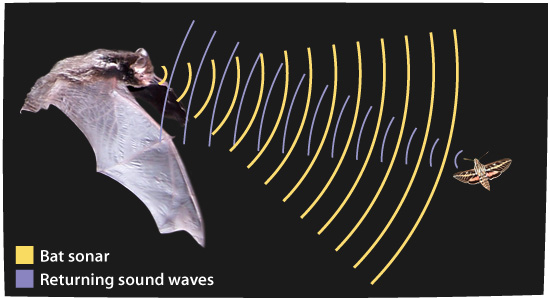
\includegraphics[width=.6\textwidth]{echolocation}
    \end{center}

    \pause
    \begin{columns}[T,onlytextwidth]
        \column{.333\textwidth}
        \begin{center}
            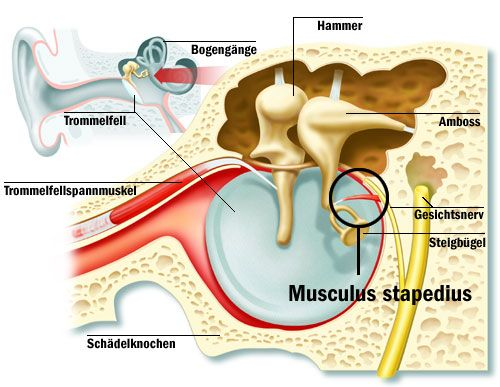
\includegraphics[width=\textwidth]{stapedius}
        \end{center}

        \pause

        \column{.333\textwidth}
        \begin{center}
            \vfill
            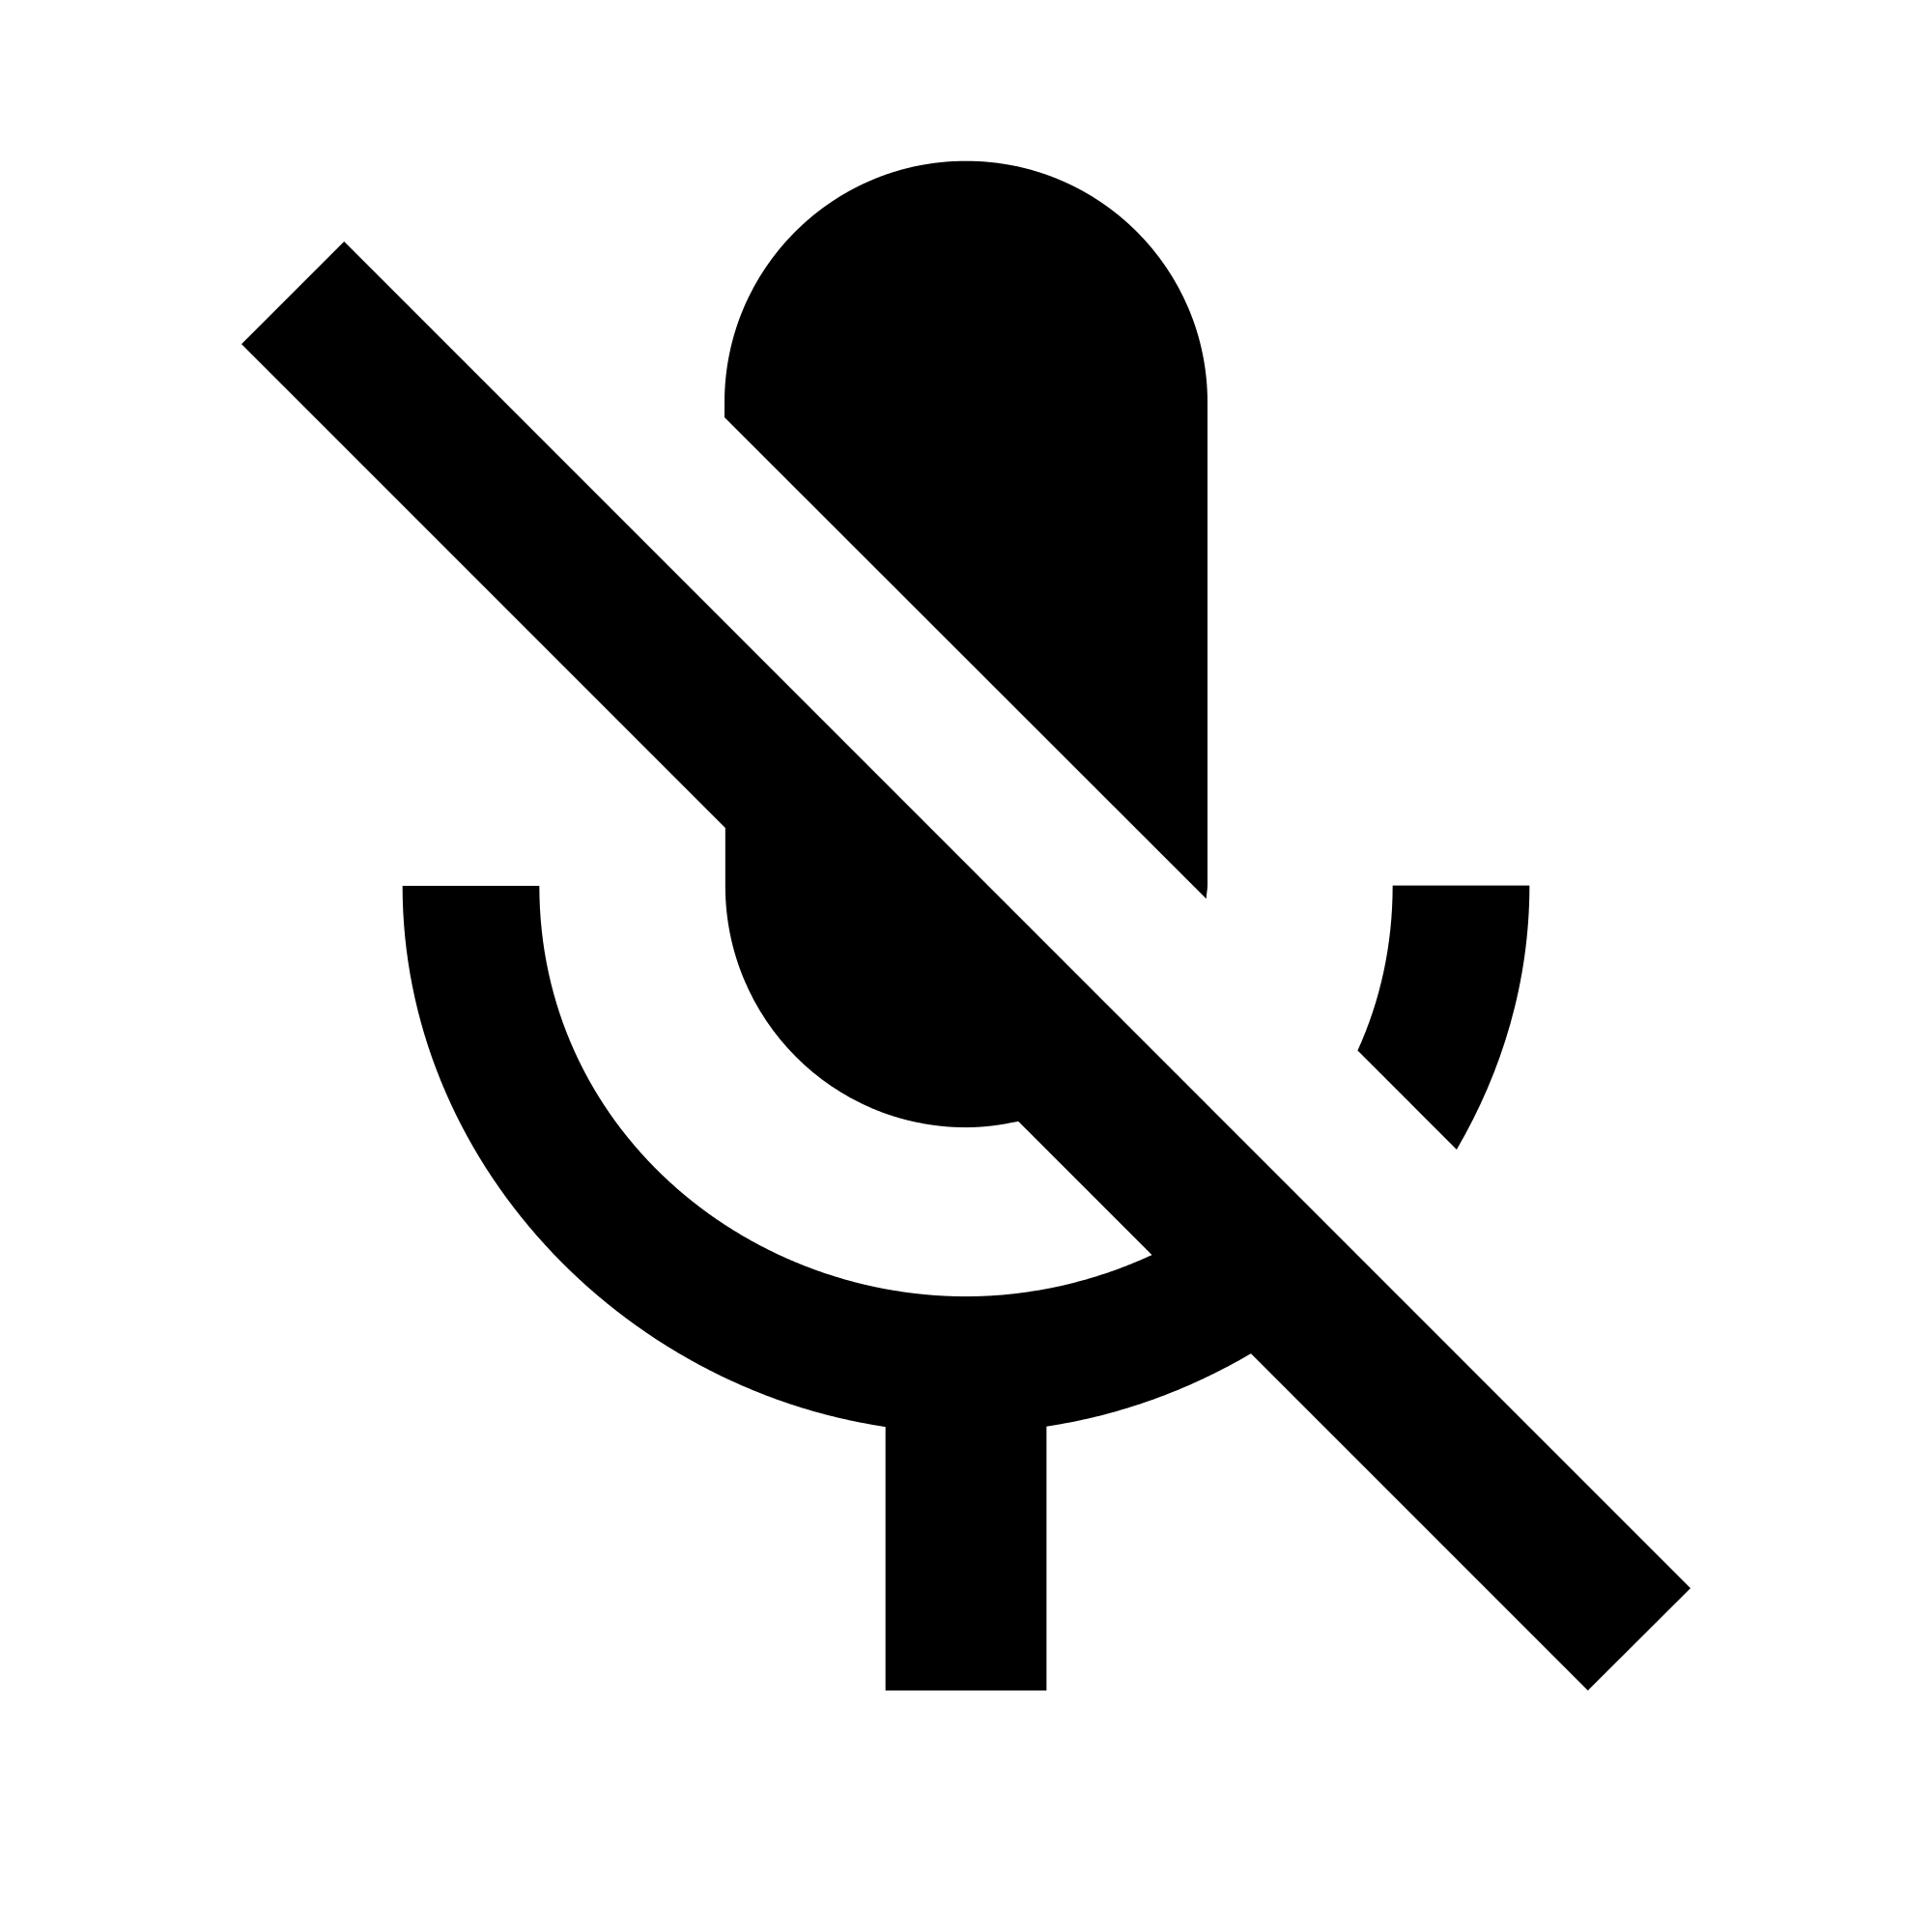
\includegraphics[width=.8\textwidth]{mute}
        \end{center}

        \pause

        \column{.333\textwidth}
        \begin{center}
            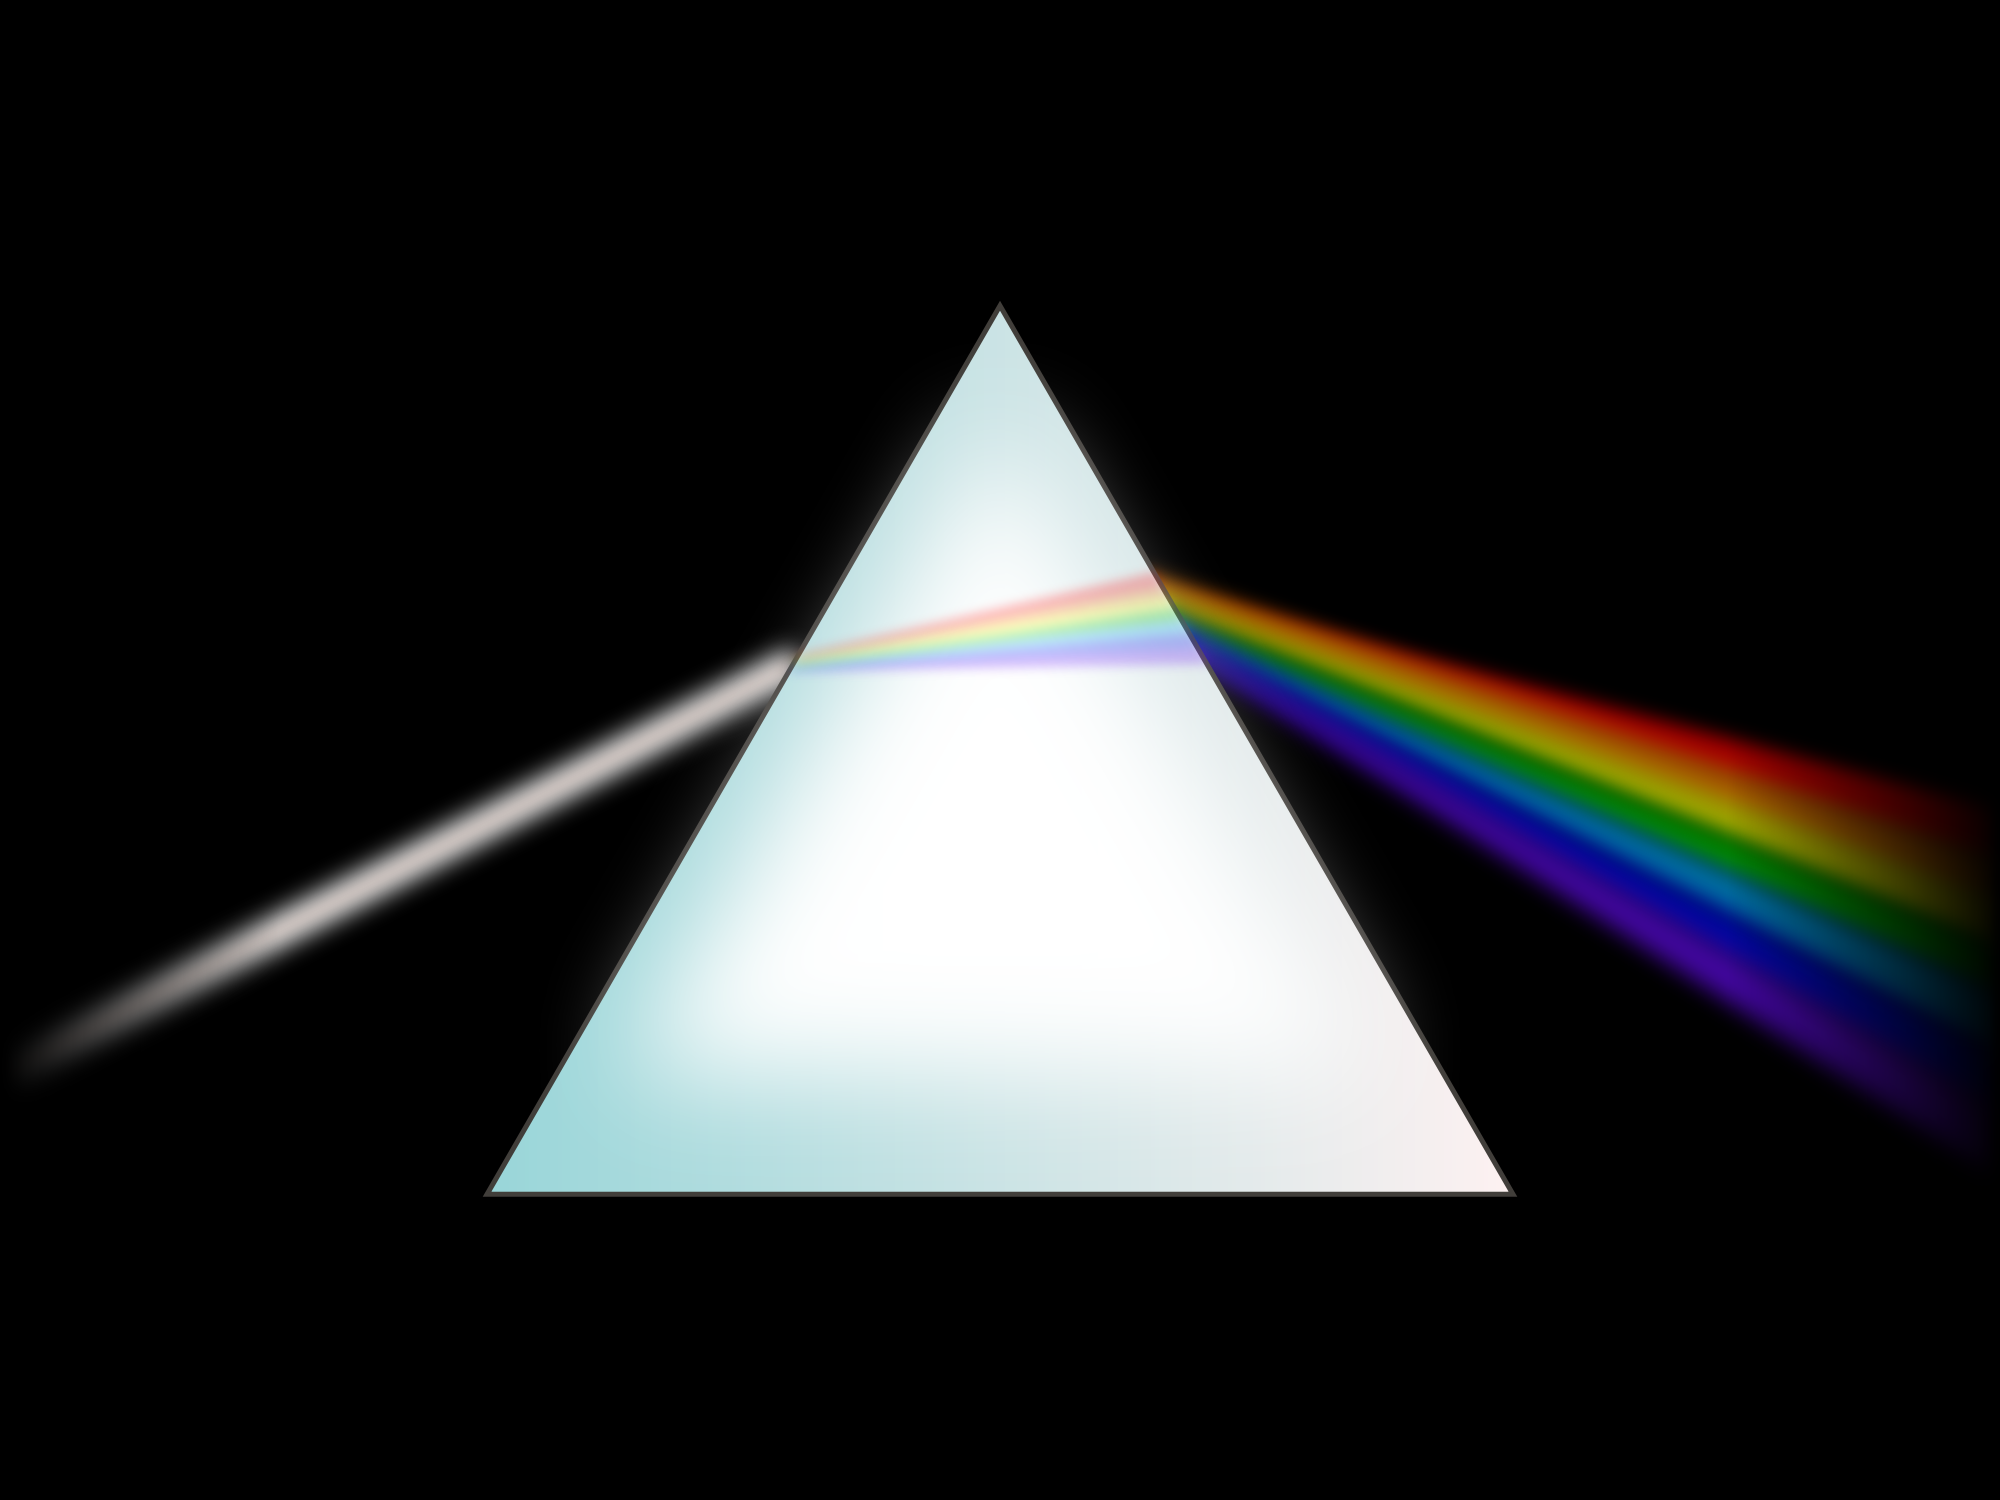
\includegraphics[width=1\textwidth]{spectrum}
        \end{center}
    \end{columns}
\end{frame}

\begin{frame}
    \frametitle{Eliminando o Auto-Bloqueio}

    Solução do artigo:
    \begin{itemize}
        \item Hardware e software \alert{co-design}
        \item Nova tag RFID: \alert{reflete harmônicos} do sinal recebido
        \item Algoritmo HMFCW: seleciona \alert{grupos de frequências}
    \end{itemize}

    \pause

    \begin{center}
        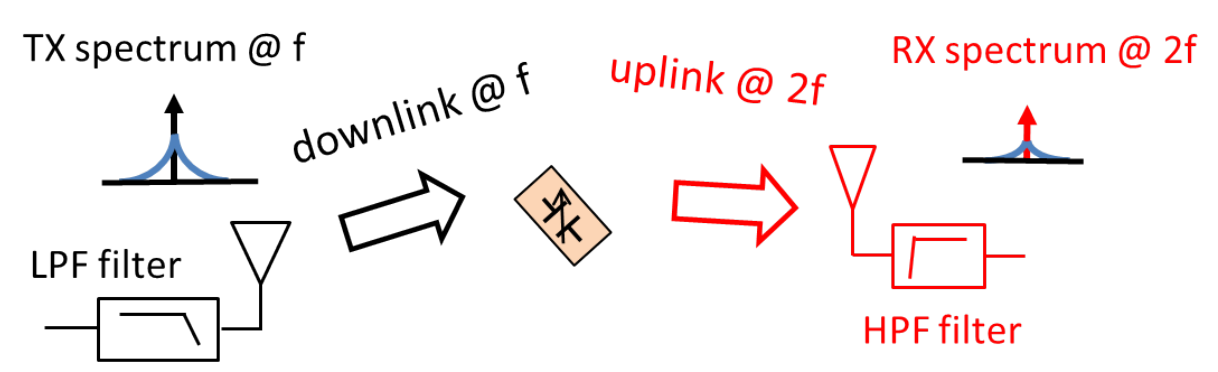
\includegraphics[width=.8\textwidth]{nonlinear-secondharmonic}
    \end{center}
\end{frame}

\section{Determinando a Variação de Frequências}
\begin{frame}
    \frametitle{Determinando a Variação de Frequências}

\end{frame}

\begin{frame}
    \frametitle{Determinando a Variação de Frequências}

\end{frame}

\section{Algoritmo de Localização 3D}
\begin{frame}
    \frametitle{Algoritmo de Localização 3D}

\end{frame}

\begin{frame}
    \frametitle{Algoritmo de Localização 3D}

\end{frame}
